\chapter{Teoría de bandas}

El modelo de enlaces permite visualizar de manera sencilla la cantidad de enlaces completos y enlaces rotos, y describir la ubicación espacial de los enlaces y de los portadores dentro de un sólido. Sin embargo, en el modelo de enlaces no se muestra información sobre las energías de las partículas. Dos electrones libres pueden tener distintos niveles energéticos, mientras que los electrones que permanecen enlazados tienen niveles de energía completamente diferentes. Para romper un enlace covalente se requiere aplicar una energía igual a la energía de la banda prohibida, $E_g$, pero hasta este momento no se ha explicado cómo se define la banda prohibida, y surge la pregunta: ¿qué es una banda de energía?

Para poder ampliar estos conceptos y explicar el comportamiento del cristal en términos de la energía, es necesario un nuevo modelo que aporte información sobre las energías de los electrones y huecos dentro del cristal de silicio. Este nuevo modelo es el \textbf{modelo de bandas de energía}.

\section{Energía de un electrón}

La energía de cualquier electrón en un átomo de silicio aislado se puede calcular con base en sus números cuánticos: el número cuántico principal $n$, el número cuántico azimutal $l$, el número cuántico magnético $m$, y el espín $s$. Retomando la configuración electrónica del silicio: 1s$^2$2s$^2$2p$^6$3s$^2$3p$^2$, se conoce que la energía de cualquier electrón dentro de esta estructura tiene niveles de energía discretos, es decir, están cuantizados.

La energía de un electrón depende de su momento angular, y por lo tanto, existen ciertos niveles de energía que pueden ocupar los electrones en cada órbita. Estos niveles de energía se pueden representar de acuerdo con el número cuántico principal \textit{n}, el cual es un número entero que pertenece a los números naturales. La energía de unión de un electrón con el núcleo de un átomo de hidrógeno se calcula mediante la ecuación:

\[E(n) = \dfrac{-13.6\ eV}{n^2}\]

Donde $n$ puede tomar valores como 1, 2, 3, etc. La unidad de medida para la energía de un electrón es el electronvoltio ($1\ eV = 1.602\times{}10^{-19}\ J$).

Observe que un electrón ubicado a una distancia infinita del núcleo tendrá una energía de cero. Este nivel energético se denomina \textbf{nivel de vacío}, y es la energía de referencia. Cualquier electrón que esté cerca del núcleo tendrá necesariamente una energía menor que el nivel de vacío. Un concepto similar es el potencial: la diferencia de potencial entre dos puntos siempre se mide con respecto a una referencia. Los electrones con energía baja están fuertemente ligados al núcleo, y se denominan \textbf{electrones del núcleo}, mientras que los electrones de las órbitas exteriores pueden formar enlaces químicos covalentes, y se denominan \textbf{electrones de valencia}. El hidrógeno tiene un electrón de valencia, y el silicio tiene cuatro.


\section{Principio de construcción}

El principio de construcción (Aufbau) permite distribuir a los electrones en los orbitales. Los orbitales se van llenando de menor energía a mayor energía. Para construir la configuración electrónica, se colocan los electrones hasta que los orbitales se llenan, y luego se pasa al siguiente orbital. En cada orbital s se pueden colocar hasta dos electrones, en los orbitales p se ubican 6, en los orbitales d se ubican 10, en los orbitales f se ubican 14, y así sucesivamente, como se observa en la Figura \ref{principio_aufbau}.

\begin{figure}[H]
    \centering
    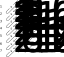
\includegraphics{figuras/principio_de_aufbau.pdf}
    \caption{Principio de construcción.}
    \label{principio_aufbau}
\end{figure}

Cuanto más cerca del núcleo de un átomo se encuentren los electrones, menor energía potencial poseen. La nube electrónica de un átomo se organiza por niveles de energía, representados por el principal número cuántico, n; que equivale a la energía del nivel o distancia respecto al núcleo del átomo. En ausencia de energía térmica, es decir, cuando se alcanzan los cero Kelvin; los catorce electrones del silicio se distribuyen por niveles de energía de la siguiente forma:

\begin{itemize}
\item 2 electrones en el primer nivel: $1s^2$
\item 8 electrones en el segundo nivel: $2s^2 2p^6$
\item 4 electrones en el tercer nivel: $3s^2 3p^2$
\end{itemize}

La configuración electrónica del silicio es $1s^{2}2s^{2}2p^{6}3s^{2}3p^{2}$ donde el número antes de cada letra es el número cuántico principal, la letra describe el tipo de orbital, y el exponente indica el número de electrones que están presentes en cada orbital. Los orbitales son las formas geométricas que describen las regiones de probabilidad de encontrar un electrón. Para construir la configuración electrónica de cualquier átomo se utiliza el principio de construcción (Aufbau).


\newpage
\section{Principio de exclusión de Pauli}

El principio de exclusión de Pauli \cite{b4} establece que no puede haber dos electrones con la misma energía, es decir, con todos los números cuánticos idénticos. Los electrones de un átomo están restringidos a un único espacio de ocupación, lo cual define que si ya un espacio está ocupado por un electrón, no existe otro electrón en el mismo átomo que esté descrito por el mismo numero cuántico, es decir, difieren en al menos el número cuántico de espín (s).  

Descrito lo anterior, si por ejemplo la probabilidad de ocupación de un electrón de un átomo específico, está definida por los números cuánticos $n=2$, $l=1$, $m=-1$, $s=1/2$; a lo sumo la combinación más similar será la que posee un $s=-1/2$ y el resto de números iguales.


\section{Modelo de bandas de energía}

Los electrones de un átomo aislado tienen niveles de energía discretos. Al acercar dos átomos, los niveles energéticos deben ser ligeramente distintos, y cuando se tiene una cantidad muy alta de átomos, la separación entre los niveles energéticos se vuelve tan pequeña que para efectos prácticos es una banda continua. Esto se observa en la Figura \ref{formacion_bandas}.

\begin{figure}[H]
    \centering
    \begin{tikzpicture}
    % Ejes
    \draw[-to] (0,0) -- (12,0);
    \draw[-to] (0,0) -- (0,8);
    \draw (0,8) node[above] {Energía};
    \draw (12,0) node[right] {Átomos};
    % Rotulos eje X
    \draw (2,-0.2) -- (2,0);
    \draw (2,-0.2) node[below] {$1$};
    \draw (4,-0.2) -- (4,0);
    \draw (4,-0.2) node[below] {$2$};
    \draw (6,-0.2) -- (6,0);
    \draw (6,-0.2) node[below] {$3$};
    \draw (9,-0.2) -- (9,0);
    \draw (9,-0.2) node[below] {$10^{23}$};
    % Rotulos eje Y
    \draw (-0.2,1.5) -- (0,1.5);
    \draw (-0.2,1.5) node[left] {$E_1$};
    \draw (-0.2,3.5) -- (0,3.5);
    \draw (-0.2,3.5) node[left] {$E_2$};
    \draw (-0.2,6) -- (0,6);
    \draw (-0.2,6) node[left] {$E_3$};
    % Energias de un atomo
    \draw (1.5,1.5) -- (2.5,1.5);
    \draw (1.5,3.5) -- (2.5,3.5);
    \draw (1.5,6) -- (2.5,6);
    % Energias de 2 atomos
    \draw (3.5,1.4) -- (4.5,1.4);
    \draw (3.5,1.6) -- (4.5,1.6);
    \draw (3.5,3.4) -- (4.5,3.4);
    \draw (3.5,3.6) -- (4.5,3.6);
    \draw (3.5,5.9) -- (4.5,5.9);
    \draw (3.5,6.1) -- (4.5,6.1);
    % Energias de 3 atomos
    \draw (5.5,1.35) -- (6.5,1.35);
    \draw (5.5,1.50) -- (6.5,1.50);
    \draw (5.5,1.65) -- (6.5,1.65);
    \draw (5.5,3.35) -- (6.5,3.35);
    \draw (5.5,3.50) -- (6.5,3.50);
    \draw (5.5,3.65) -- (6.5,3.65);
    \draw (5.5,5.85) -- (6.5,5.85);
    \draw (5.5,6.00) -- (6.5,6.00);
    \draw (5.5,6.15) -- (6.5,6.15);
    % Bandas de energia continuas
    \draw (8.5,1.2) rectangle (9.5,1.8);
    \draw (8.5,3.2) rectangle (9.5,3.8);
    \draw (8.5,5.7) rectangle (9.5,6.3);
    \end{tikzpicture}
    \caption{Formación de bandas de energía continuas en sólidos.}
    \label{formacion_bandas}
\end{figure}

Se sabe que un cristal de silicio está compuesto por N átomos del elemento, que de alguna forma se han acercado lo suficiente como para conformar una sola estructura \cite{b4}\cite{b7}. En un sólido con enlace covalente, como lo es un cristal de silicio, los niveles energéticos se convierten en bandas continuas. El espaciamiento reticular de las celdas unitarias de un cristal de silicio, conocido como ``\textit{lattice paramter}'', es de 5.43 \AA\, y la distancia mínima interatómica en equilibrio es de 2.35 \AA.


\section{Diagrama de bandas en equilibrio}

Los N átomos de silicio analizados de forma aislada tienen 6N estados p y 2N estados s. El último y más alto nivel de energía potencial, tiene 8N estados posibles y 4N electrones. En un cristal, los 8N estados convergen a 4N estados vacíos y a 2N + 2N estados ocupados, de acuerdo con su distribución energética de átomos separados. El grupo de estados ocupados se llama nivel de valencia y posee a los electrones del átomo con mayor nivel de energía potencial \cite{b7}\cite{b11}. Los electrones de valencia son los que determinan la forma en que el elemento se relaciona e interactúa con el entorno. 

El nivel de energía $E_{v}$ representa el máximo energético bajo el cual se ubican los electrones de valencia, definiendo así a la \textbf{banda de valencia} de un semiconductor. La \textbf{banda de conducción} se define al buscar un nivel energético superior al de la banda de valencia donde los estados están vacíos. En esta banda se define un valor mínimo $E_{c}$. Existe una brecha entre ambas bandas, denominada \textbf{banda prohibida}, y conceptualmente expresa la cantidad de energía necesaria para que un electrón se mueva desde la banda de valencia hacia la de conducción. 

Al analizar los niveles energéticos de las bandas formadas en un sólido, surgen un conceptos como lo es el nivel de vacío ($E_{vac}$) \cite{b4}, que es donde la energía potencial alcanza su valor máximo, en cero. Un electrón requiere sobrepasar dicho valor para escapar del sólido, en ese punto su energía es únicamente cinética.

La diferencia energética entre el nivel mínimo de la banda de conducción $E_{c}$ y el nivel de vacío $E_{vac}$, establece el valor de la afinidad electrónica ($\chi$) para los dispositivos semiconductores. Por otro lado, el esfuerzo que debe de realizar un electrón desde el nivel de Fermi ($E_{F}$) \cite{b11} para liberarse del semiconductor, se llama función de trabajo ($\phi$).

El diagrama de bandas de energía para el silicio tipo n se muestra en la Figura \ref{diagrama_bandas_silicio}. 

\begin{figure}[H]
    \centering
    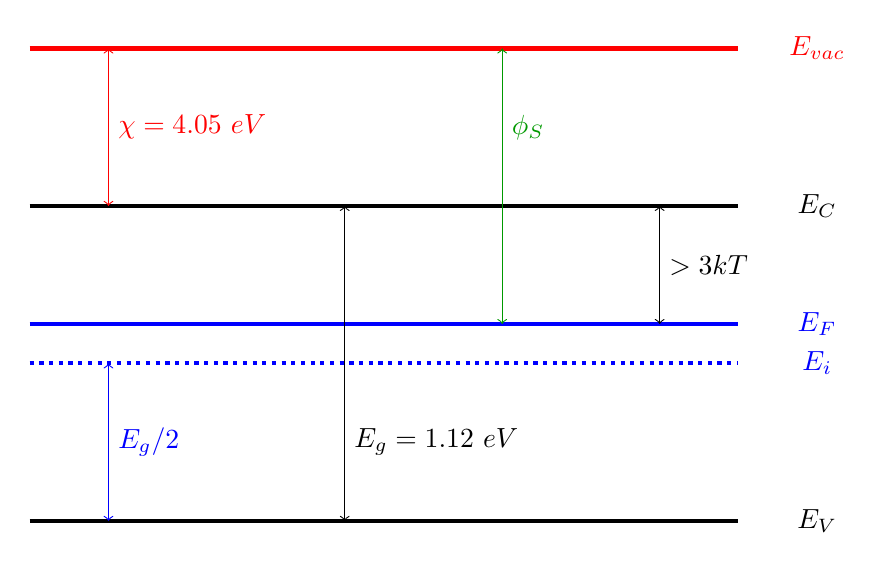
\begin{tikzpicture}
    % Nivel de vacio
    \draw[color=red,line width=1.5pt] (0,0) -- (9,0);
    \node[color=red] at (10,0) {$E_{vac}$};
    % Banda conduccion
    \draw[color=black,line width=1.5pt] (0,-2) -- (9,-2);
    \node[color=black] at (10,-2) {$E_{C}$};
    % Nivel Fermi
    \draw[color=blue,line width=1.5pt] (0,-3.5) -- (9,-3.5);
    \node[color=blue] at (10,-3.5) {$E_{F}$};
    % Nivel Fermi intrinseco
    \draw[dotted,color=blue,line width=1.5pt] (0,-4) -- (9,-4);
    \node[color=blue] at (10,-4) {$E_{i}$};
    % Banda valencia
    \draw[color=black,line width=1.5pt] (0,-6) -- (9,-6);
    \node[color=black] at (10,-6) {$E_{V}$};
    % Afinidad electronica
    \draw[to-to,color=red] (1,0) -- node[right] {$\chi=4.05\ eV$} (1,-2);
    % Funcion de trabajo
    \definecolor{darkgreen}{rgb}{0,0.6,0}
    \draw[to-to,color=darkgreen] (6,0) -- (6,-3.5);
    \draw[color=darkgreen] (6,-1) node[right] {$\phi_S$};
    % Banda prohibida
    \draw[to-to,color=black] (4,-2) -- (4,-6);
    \draw[color=black] (4,-5) node[right] {$E_g = 1.12\ eV$};
    % Dopado degenerado
    \draw[to-to,color=black] (8,-2) -- (8,-3.5);
    \draw[color=black] (8,-2.75) node[right] {$> 3kT$};
    % Media banda prohibida
    \draw[to-to,color=blue] (1,-4) -- (1,-6);
    \draw[color=blue] (1,-5) node[right] {$E_g/2$};
    \end{tikzpicture}
    \caption{Diagrama de bandas de energía del silicio tipo n en equilibrio térmico.}
    \label{diagrama_bandas_silicio}
\end{figure}



En la Tabla \ref{tabla_constantes_1} se resumen algunas constantes para semiconductores que son comúnmente utilizados en la industria microelectrónica. En la Tabla \ref{tabla_constantes_2} se resumen las funciones de trabajo de varios metales.

\begin{table}[H]
    \centering
    \caption{Constantes para semiconductores comunes.}
    \label{tabla_constantes_1}
    \begin{tabular}{|c|c|c|}
        \hline \textbf{Material} & \textbf{$\chi$} & \textbf{$E_g$} \\
        \hline Silicio & 4.05 eV & 1.12 eV \\
        Germanio & 4.13 eV & 0.66 eV \\
        GaAs & 4.07 eV & 1.42 eV \\
        \hline
    \end{tabular}
\end{table}

\begin{table}[H]
    \centering
    \caption{Funciones de trabajo para metales comunes.}
    \label{tabla_constantes_2}
    \begin{tabular}{|c|c|}
        \hline \textbf{Material} & \textbf{$\phi_M$} \\
        \hline 
        Níquel      & 5.15 eV \\
        Oro         & 5.10 eV \\
        Molibdeno   & 4.60 eV \\
        Tungsteno   & 4.55 eV \\
        Cromo       & 4.50 eV \\
        Aluminio    & 4.28 eV \\
        Plata       & 4.26 eV \\
        \hline
    \end{tabular}
\end{table}

\newpage
\begin{ejemplo}
Dibuje el diagrama de bandas de energía de los siguientes materiales: silicio, oro, germanio y tungsteno. Indique los valores numéricos para la función de trabajo, afinidad electrónica, energía de la banda prohibida y la posición del nivel de Fermi.
\end{ejemplo}

\begin{solucion}
El diagrama de bandas de cada uno de los materiales se muestra a continuación:

\begin{figure}[H]
    \centering
    \includegraphics{figuras/bandas_solucion_ejemplo1.png}
    \caption{Solución: diagrama de bandas de materiales aislados en equilibrio.}
    \label{diagrama_bandas_solucion}
\end{figure}
\end{solucion}


\newpage
\section{Densidad de estados}

En cada una de las bandas de energía existe una cierta cantidad de estados disponibles, que pueden ser ocupados por electrones libres en la banda de conducción, o por huecos libres en la banda de valencia. La distribución de la densidad de estados en función de la energía se calcula con las siguientes ecuaciones:

\[ g_c(E) = \dfrac{m_n \sqrt{2m_n (E-E_c)}}{\pi^2 h^3}\ \ \ \ \ E \geq E_c \]

\[ g_v(E) = \dfrac{m_p \sqrt{2m_p (E_v-E)}}{\pi^2 h^3}\ \ \ \ \ E \leq E_v \]

Lo anterior es una distribución de estados en energía que permite determinar de cuantos estados se dispone a determino valor de energía. Es claro que entre más bajo sea el valor de energía respecto a $E_{v}$, mayor disponibilidad de espacio tienen los huecos. Por otro lado, entre más supere el valor de energía al valor de $E_{c}$, mayor disponibilidad de espacio tendrán los electrones.

La densidad de estados se puede representar con una analogía: en un estadio, la cantidad de asientos disponibles en cada una de las graderías es limitada, y las personas pueden ocupar sólo esta cantidad de asientos. 

\section{Distribución de Fermi-Dirac}

La función de densidad de probabilidad de Fermi-Dirac indica la probabilidad de ocupación de un estado energético con energía E. La probabilidad de ocupación para electrones es $f(E)$, y para huecos $h(E)$:

\[ f(E) = \dfrac{1}{1 + e^{\dfrac{E-E_F}{kT}}} \]

\[ h(E) = 1 - \dfrac{1}{1 + e^{\dfrac{E-E_F}{kT}}} \]

El \textbf{nivel de Fermi} se define como el nivel energético donde la probabilidad de ocupación es del 50\% para ambos electrones y huecos. En un semiconductor intrínseco, el nivel de Fermi se posiciona exactamente en la mitad de la banda prohibida, a una misma distancia de la banda de conducción y de la banda de valencia. En los diagramas de bandas de energía, la mitad de la banda se denota con una línea punteada rotulada como $E_i$, indicando la posición del nivel de Fermi intrínseco.

Siguiendo con la analogía del estadio, las personas en un estadio tienen cierta preferencia por los mejores asientos, por ejemplo, aquellos que no estén expuestos al sol y que tengan buena visibilidad a la gramilla. Lo mismo sucede con los electrones y los huecos: la densidad de estados indica cuántos asientos disponibles existen, mientras que la distribución de Fermi-Dirac indica cuál es la preferencia de los electrones y huecos por ocupar los ``asientos'' disponibles de la densidad de estados.

%La temperatura afecta la forma que tiene la función de Fermi. Cuando la temperatura es cercana a 0 K, la función de Fermi toma valores de 0 o 1. Un 0 significa que la probabilidad de ocupación es nula, mientras que un 1 indica una probabilidad del 100\% o total certeza. Esto significa que a 0 K, por debajo de $E_F$ todos los estados electrónicos están llenos, y por encima de $E_F$ todos los estados electrónicos están vacíos.



%\section{Portadores en silicio}

% NOTA: comento esta sección porque creo que en realidad las concentraciones son las integrales de los productos de g x f, integrando desde el borde de la banda hasta infinito. Hay que revisarlo.


%La concentración de electrones por unidad de volumen puede calcularse como el producto de la densidad de estados por la probabilidad de ocupación de estados. Matemáticamente:

%\[ n = g_c(E) f(E) \]

%De la misma manera, la concentración de huecos es:

%\[ p = g_v(E) h(E) \]


\section{Concentraciones de portadores}

El dopado puede mover el nivel de Fermi a posiciones distintas del nivel de Fermi intrínseco. Se dijo anteriormente que, en un \textbf{semiconductor intrínseco}, el nivel de Fermi está ubicado exactamente en la mitad de la banda prohibida. En un \textbf{semiconductor extrínseco}, si el nivel de Fermi está por encima del nivel de Fermi intrínseco, el semiconductor es de tipo n, y se cumple que:

\[ E_F - E_i =  kT \ln \dfrac{N_D}{n_i} \]

\[ n = n_i \cdot e^{\dfrac{E_F-E_i}{kT}} \]

Si el nivel de Fermi está por debajo del nivel de Fermi intrínseco, el semiconductor es de tipo p, y:

\[ E_i - E_F =  kT \ln \dfrac{N_A}{n_i} \]

\[ p = n_i \cdot e^{\dfrac{E_i-E_F}{kT}} \]

\begin{ejemplo}
Una oblea de silicio está dopada con boro, con una concentración $N_A=10^{15}\ cm^{-3}$. 

\begin{itemize}
    \item Determine la posición del nivel de Fermi con respecto al nivel de Fermi intrínseco.
\end{itemize}

La oblea del caso anterior se dopa adicionalmente con arsénico, donde se implanta una concentración de átomos de arsénico de $N_D=2.1 \times 10^{15}\ cm^{-3}$. Bajo estas condiciones indique:

\begin{itemize}
    \item El nivel de dopado efectivo resultante.
    \item La concentración de portadores (n y p) resultante.
    \item La nueva posición del nivel de Fermi $E_F$ con respecto a $E_i$.
\end{itemize}

\end{ejemplo}

\begin{solucion}
(En clase).
\end{solucion}


%\begin{ejemplo}
%En una muestra de silicio intrínseco a temperatura ambiente, la probabilidad de ocupación de electrones en un determinado nivel de energía $E_X$ es del 58\%. 

%\begin{enumerate}
%    \item Determine la posición de ese nivel de energía $E_X$ con respecto al nivel de Fermi intrínseco.
%    \item Calcule la probabilidad de ocupación de huecos en ese mismo nivel de energía mencionado.
%    \item Dibuje el diagrama de bandas de energía, indicando el nivel energético que tiene la probabilidad de ocupación de electrones propuesta.
%    \item Si la muestra de silicio intrínseco está a T = 0 K, indique la probabilidad de ocupación de electrones que existe en el nivel de energía calculado anteriormente.
%\end{enumerate}
%\end{ejemplo}

%\begin{solucion}
%(En clase).
%\end{solucion}

\newpage
\section{Semiconductores degenerados}

Si el nivel de Fermi se acerca a alguna de las bandas, a una distancia menor que $3kT$, se dice que es un \textbf{semiconductor degenerado} ya que el dopado es muy intenso, lo que ocasiona que el material pierda sus propiedades semiconductoras y se parezca más a un metal. En la fabricación de semiconductores, se utiliza silicio con altas concentraciones de dopado en la compuerta de los transistores MOSFET, que antes era metálica y en la actualidad se ha reemplazado por silicio policristalino altamente dopado.

La concentración de dopado degenerado para silicio se puede calcular con el siguiente ejemplo.

\begin{ejemplo}
Calcule cuál es la concentración máxima de átomos donadores que se puede agregar a una muestra de silicio intrínseco, para que el material siga siendo no degenerado.
\end{ejemplo}

\begin{solucion}
La condición que se debe cumplir es:

\[ E_C - E_F > 3kT \]

Donde la banda de conducción se puede reescribir como $E_i+E_g/2$:

\[ (E_i + E_g/2) - E_F > 3kT \]

\[ E_i - E_F > 3kT - E_g/2 \]

Para semiconductores N se conoce además que:

\[ E_F - E_i = kT \ln \dfrac{N_D}{n_i }\]

La equivalencia queda entonces:

\[ -kT \ln \dfrac{N_D}{n_i} > 3kT - \dfrac{E_g}{2} \]

\[ \ln \dfrac{N_D}{n_i} < \dfrac{E_g}{2kT} - 3 \]

De donde se resuelve:
\[ N_D < n_i \cdot e^{ \left( \dfrac{E_g}{2kT} - 3 \right) } \]

\[ N_D < (10^{10}) \cdot e^{ \left( \dfrac{1.12\ eV}{2(26\ meV)} - 3 \right) } \]

La concentración máxima permitida de átomos donadores en silicio no degenerado es:

\[ N_D < 1.125 \times 10^{18}\ cm^{-3} \]
\end{solucion}

%\newpage
%\section*{Problemas}

%\textbf{Problema 2.1.} Dibuje el diagrama de bandas de energía para silicio intrínseco a temperatura ambiente. Indique la posición del nivel de Fermi, la banda de conducción, la banda de valencia, el nivel de vacío, la función de trabajo y la afinidad electrónica.

%\textbf{Problema 2.2.} Calcule la posición del nivel de Fermi con respecto al nivel de Fermi intrínseco para los materiales que se presentan a continuación. Dibuje el diagrama de bandas de energía para cada caso.

%\begin{enumerate}
%\item Silicio dopado con $N_D=2\times{}10^{15}\ cm^{-3}$.
%\item Silicio dopado con $N_A=3.1\times{}10^{15} cm^{-3}$.
%\item Silicio con ambos dopados $N_D=2\times{}10^{15}\ cm^{-3}$ y $N_A=3.1\times{}10^{15} cm^{-3}$.
%\end{enumerate}


